\documentclass[aspectratio=169,10pt]{beamer}
% ===================================================================
%  v7 Householder QR — animated step-by-step dry run (Beamer)
%  Build:  cd docs && tectonic v7_walkthrough_slides.tex
%  Each frame uses overlays (\onslide / \only / \alt) so a PDF viewer
%  in presentation mode "animates": click to reveal the next sub-step.
% ===================================================================
\usetheme{Madrid}
\usecolortheme{seahorse}
\useinnertheme{circles}
\setbeamertemplate{navigation symbols}{}
\setbeamertemplate{caption}[numbered]

\usepackage{amsmath,amssymb}
\usepackage{tikz}
\usetikzlibrary{matrix,backgrounds,arrows.meta,positioning,calc,fit,decorations.pathreplacing,shapes.geometric}
\usepackage{booktabs}

\definecolor{critcol}{RGB}{210,60,50}
\definecolor{workcol}{RGB}{45,110,190}
\definecolor{okgreen}{RGB}{20,140,70}
\definecolor{hl}{RGB}{255,214,90}

\newcommand{\vt}{v^{\!\top}}
\newcommand{\crit}[1]{\textcolor{critcol}{#1}}
\newcommand{\work}[1]{\textcolor{workcol}{#1}}

% highlight column #2 of a tikz matrix named M, on overlay spec #1, color #3.
% Overlay-aware boxed outline drawn on the main layer (robust beamer+tikz);
% no fill/transparency/background-layer, which were the fragile parts.
\newcommand{\colhi}[3]{%
  \draw<#1>[#3,very thick,rounded corners=2pt]
    (M-1-#2.north west) rectangle (M-4-#2.south east);}

\title[v7 DAG-HVX QR]{Householder QR with DAG-Priority HVX Scheduling}
\subtitle{An animated, step-by-step dry run of \texttt{v7\_dag\_hvx\_sched}}
\author{QR-on-Hexagon research notes}
\date{\today}

\begin{document}

% ---------------------------------------------------------------
\begin{frame}\titlepage\end{frame}

% ---------------------------------------------------------------
\begin{frame}{What this deck does}
We factor a small matrix $A=QR$ \emph{by hand}, exactly as the code does, one click
at a time.
\begin{itemize}
  \item \crit{Red} = the \textbf{critical path} (reflector $\to$ next column $\to$ next reflector).
  \item \work{Blue} = \textbf{parallel} trailing-column updates handed to worker threads.
  \item Each step does a tiny change to the matrix; watch the upper triangle ($R$) fill in.
\end{itemize}
\vfill
\begin{block}{The running example ($4\times3$)}
\[
A=\begin{bmatrix} 4&-2&1\\ 0&6&-1\\ 3&1&2\\ 0&2&4\end{bmatrix}
\]
\end{block}
\end{frame}

% ---------------------------------------------------------------
\begin{frame}{The math of one reflector (reference card)}
For column $k$, with $x=A[k{:}m,\,k]$:
\begin{align*}
\alpha &= -\operatorname{sign}(x_k)\,\lVert x\rVert, &
v &= x-\alpha e_1\ \ (\text{i.e. } v_k \mathrel{-}=\alpha),\\
\tau &= \frac{2}{\vt v}, &
H_k a &= a - \underbrace{\tau(\vt a)}_{w}\,v .
\end{align*}
\begin{itemize}
  \item One \textbf{reduction} ($\vt a$, a dot product) + one \textbf{saxpy} ($a\mathrel{-}=w v$) per column.
  \item The diagonal becomes $\alpha$; everything below it is annihilated.
\end{itemize}
\end{frame}

% ===============================================================
%  STEP 0
% ===============================================================
\begin{frame}{Step $k=0$ \quad (animate: click through the sub-steps)}
\begin{columns}[T]
\begin{column}{0.46\textwidth}
\centering
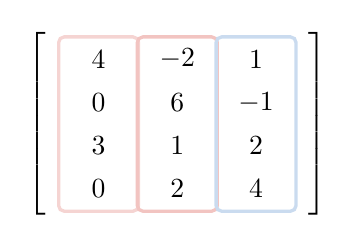
\begin{tikzpicture}
\matrix (M) [matrix of math nodes, ampersand replacement=\&, left delimiter={[},right delimiter={]},
  nodes={minimum width=1.0cm,minimum height=0.55cm,anchor=center}]{
  4 \& -2 \& 1 \\ 0 \& 6 \& -1 \\ 3 \& 1 \& 2 \\ 0 \& 2 \& 4 \\};
\colhi{2-}{1}{critcol!22}   % pivot column highlighted from sub-step 2
\colhi{6-}{2}{critcol!30}   % critical col 1
\colhi{7-}{3}{workcol!25}   % worker col 2
\end{tikzpicture}

\medskip
\footnotesize\onslide<2->{pivot column $x=(4,0,3,0)$}
\end{column}
\begin{column}{0.54\textwidth}
\small
\begin{itemize}\itemsep4pt
  \item<3-> $\lVert x\rVert=\sqrt{16+9}=\mathbf{5}$,\quad $x_0=4\ge0 \Rightarrow \alpha=\crit{-5}$
  \item<4-> $v = x-\alpha e_1 = (4{-}({-}5),0,3,0)=\crit{(9,0,3,0)}$
  \item<5-> $\vt v = 81+9 = 90$,\quad $\tau=\tfrac{2}{90}=\mathbf{0.0222}$
  \item<6-> \crit{Critical col 1}: $\vt a=-15,\ w=\tau\,(-15)=-0.333$\\
        $(-2,6,1,2)\to\crit{(1,6,2,2)}$
  \item<7-> \work{Worker col 2}: $\vt a=15,\ w=0.333$\\
        $(1,-1,2,4)\to\work{(-2,-1,1,4)}$
  \item<8-> set diagonal $\alpha$, zero below it
\end{itemize}
\end{column}
\end{columns}
\onslide<8->{\vfill\centering\footnotesize after step 0 the first column of $R$ is done.}
\end{frame}

% result of step 0
\begin{frame}{After step $k=0$}
\centering
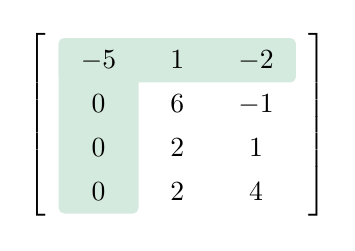
\begin{tikzpicture}
\matrix (M) [matrix of math nodes, ampersand replacement=\&, left delimiter={[},right delimiter={]},
  nodes={minimum width=1.0cm,minimum height=0.55cm}]{
  -5 \& 1 \& -2 \\ 0 \& 6 \& -1 \\ 0 \& 2 \& 1 \\ 0 \& 2 \& 4 \\};
\begin{scope}[on background layer]
  \fill[okgreen!18,rounded corners=2pt] (M-1-1.north west) rectangle (M-4-1.south east);
  \fill[okgreen!18,rounded corners=2pt] (M-1-1.north west) rectangle (M-1-3.south east);
\end{scope}
\end{tikzpicture}

\vfill
\footnotesize\textcolor{okgreen}{Green} = settled $R$ entries (column 0 and row 0).
Columns 1--2 below the diagonal still hold ``live'' data for the next steps.
\end{frame}

% ===============================================================
%  STEP 1
% ===============================================================
\begin{frame}{Step $k=1$}
\begin{columns}[T]
\begin{column}{0.46\textwidth}
\centering
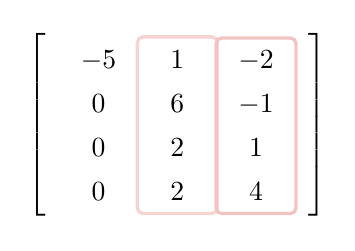
\begin{tikzpicture}
\matrix (M) [matrix of math nodes, ampersand replacement=\&, left delimiter={[},right delimiter={]},
  nodes={minimum width=1.0cm,minimum height=0.55cm}]{
  -5 \& 1 \& -2 \\ 0 \& 6 \& -1 \\ 0 \& 2 \& 1 \\ 0 \& 2 \& 4 \\};
\colhi{2-}{2}{critcol!22}
\colhi{6-}{3}{critcol!30}
\end{tikzpicture}

\medskip\footnotesize\onslide<2->{pivot $x=A[1{:},1]=(6,2,2)$}
\end{column}
\begin{column}{0.54\textwidth}
\small
\begin{itemize}\itemsep4pt
  \item<3-> $\lVert x\rVert=\sqrt{36+4+4}=\mathbf{6.633}$,\quad $\alpha=\crit{-6.633}$
  \item<4-> $v=(0,\;6{-}({-}6.633),\;2,\;2)=\crit{(0,12.633,2,2)}$
  \item<5-> $\vt v=167.60$,\quad $\tau=\mathbf{0.01193}$
  \item<6-> \crit{Critical col 2}: $\vt a=-2.633,\ w=-0.0314$\\
        $(-2,-1,1,4)\to\crit{(-2,-0.603,1.063,4.063)}$
  \item<7-> (no worker columns: $j$ ranges over $\{2\}$ only)
  \item<8-> set diagonal $\alpha$, zero below it
\end{itemize}
\end{column}
\end{columns}
\onslide<8->{\vfill\centering\footnotesize the $2\times2$ trailing block remains.}
\end{frame}

\begin{frame}{After step $k=1$}
\centering
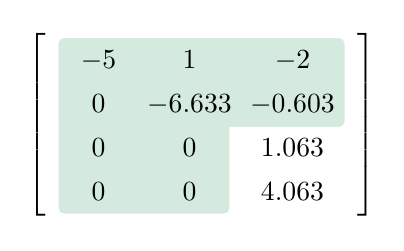
\begin{tikzpicture}
\matrix (M) [matrix of math nodes, ampersand replacement=\&, left delimiter={[},right delimiter={]},
  nodes={minimum width=1.0cm,minimum height=0.55cm}]{
  -5 \& 1 \& -2 \\ 0 \& -6.633 \& -0.603 \\ 0 \& 0 \& 1.063 \\ 0 \& 0 \& 4.063 \\};
\begin{scope}[on background layer]
  \fill[okgreen!18,rounded corners=2pt] (M-1-1.north west) rectangle (M-4-2.south east);
  \fill[okgreen!18,rounded corners=2pt] (M-1-1.north west) rectangle (M-2-3.south east);
\end{scope}
\end{tikzpicture}

\vfill
\footnotesize Columns 0--1 of $R$ done. Only the last column's $2\times2$ tail is left.
\end{frame}

% ===============================================================
%  STEP 2
% ===============================================================
\begin{frame}{Step $k=2$ (final reflector)}
\begin{columns}[T]
\begin{column}{0.46\textwidth}
\centering
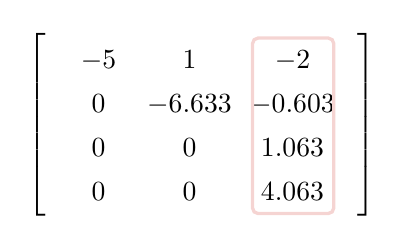
\begin{tikzpicture}
\matrix (M) [matrix of math nodes, ampersand replacement=\&, left delimiter={[},right delimiter={]},
  nodes={minimum width=1.0cm,minimum height=0.55cm}]{
  -5 \& 1 \& -2 \\ 0 \& -6.633 \& -0.603 \\ 0 \& 0 \& 1.063 \\ 0 \& 0 \& 4.063 \\};
\colhi{2-}{3}{critcol!22}
\end{tikzpicture}

\medskip\footnotesize\onslide<2->{pivot $x=A[2{:},2]=(1.063,4.063)$}
\end{column}
\begin{column}{0.54\textwidth}
\small
\begin{itemize}\itemsep4pt
  \item<3-> $\lVert x\rVert=\sqrt{1.13+16.5}=\mathbf{4.200}$,\quad $\alpha=\crit{-4.200}$
  \item<4-> $v=(0,0,\;1.063{-}({-}4.2),\;4.063)=\crit{(0,0,5.262,4.063)}$
  \item<5-> $\vt v=44.20$,\quad $\tau=\mathbf{0.04525}$
  \item<6-> no trailing columns; just place $\alpha$ and zero below
\end{itemize}
\end{column}
\end{columns}
\end{frame}

% ===============================================================
%  FINAL R
% ===============================================================
\begin{frame}{Result: $R$ (and a machine-checked cross-validation)}
\centering
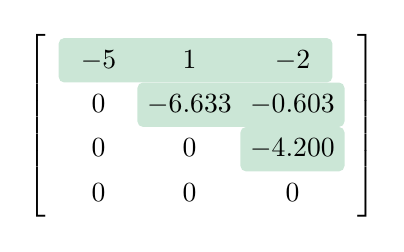
\begin{tikzpicture}
\matrix (M) [matrix of math nodes, ampersand replacement=\&, left delimiter={[},right delimiter={]},
  nodes={minimum width=1.0cm,minimum height=0.55cm}]{
  -5 \& 1 \& -2 \\ 0 \& -6.633 \& -0.603 \\ 0 \& 0 \& -4.200 \\ 0 \& 0 \& 0 \\};
\begin{scope}[on background layer]
  \fill[okgreen!22,rounded corners=2pt] (M-1-1.north west) rectangle (M-1-3.south east);
  \fill[okgreen!22,rounded corners=2pt] (M-2-2.north west) rectangle (M-2-3.south east);
  \fill[okgreen!22,rounded corners=2pt] (M-3-3.north west) rectangle (M-3-3.south east);
\end{scope}
\end{tikzpicture}

\vfill
\small
$|R|$ matches \texttt{numpy.linalg.qr} to $9\times10^{-16}$ (R is unique up to row signs).
The code checks exactly this: \texttt{max |R|-err} and the sub-diagonal residual.
\end{frame}

% ===============================================================
%  WHERE HVX FITS — the reduction, animated
% ===============================================================
\begin{frame}{Inside one update: the HVX horizontal reduction}
The dot product $\vt a$ accumulates \emph{32 partial sums} (one per lane). We still need
the scalar total --- done with 5 rotate-and-add stages, \crit{no memory traffic}.
\vfill
\centering
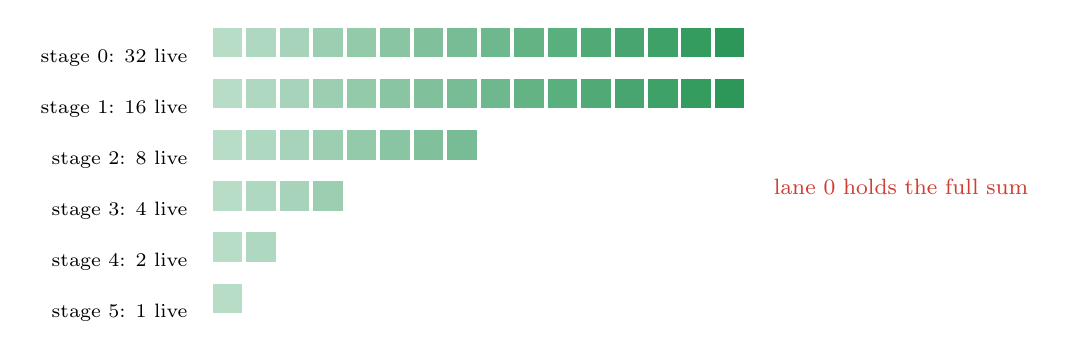
\begin{tikzpicture}[scale=0.5,every node/.style={font=\scriptsize}]
  \def\lvls{{32,16,8,4,2,1}}
  \foreach \s [count=\ov from 1] in {0,...,5} {
    \pgfmathparse{\lvls[\s]}\edef\w{\pgfmathresult}
    \onslide<\ov->{
      \node[anchor=east] at (-0.4,-1.3*\s) {\,stage \s: \w\ live};
      \foreach \b in {0,...,15} {
        \pgfmathtruncatemacro\show{ \b < \w ? 1 : 0 }
        \ifnum\show=1 \fill[okgreen!\the\numexpr30+4*\b\relax!white]
          (\b*0.85,-1.3*\s) rectangle (\b*0.85+0.75,-1.3*\s+0.75); \fi
      }
    }
  }
  \onslide<6->{\node[anchor=west,critcol,font=\footnotesize] at (14,-3.3)
    {lane 0 holds the full sum};}
\end{tikzpicture}
\vfill
\footnotesize\onslide<2->{Rotate by half the live width (\texttt{Q6\_V\_vror\_VR}, in
\emph{bytes}: 64,32,16,8,4) and add. $\log_2 32 = 5$ stages.}
\end{frame}

% ===============================================================
%  SCHEDULING — DAG critical path, animated reveal
% ===============================================================
\begin{frame}{Why ``critical path''? (reveal the DAG)}
\centering
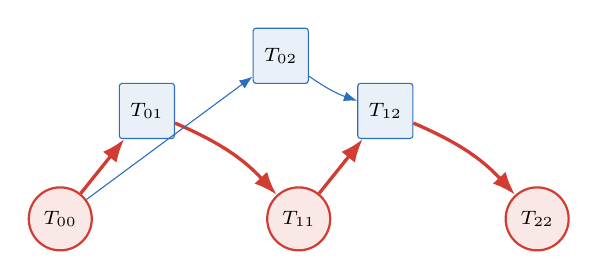
\begin{tikzpicture}[>=Latex,
  reflector/.style={circle,draw=critcol,fill=critcol!12,thick,minimum size=8mm,font=\scriptsize},
  update/.style={rectangle,draw=workcol,fill=workcol!10,minimum size=7mm,font=\scriptsize,rounded corners=1pt}]
  \node[reflector] (r0) {$T_{00}$};
  \node[reflector,right=22mm of r0] (r1) {$T_{11}$};
  \node[reflector,right=22mm of r1] (r2) {$T_{22}$};
  \node[update,above=6mm of r0,xshift=11mm] (u01) {$T_{01}$};
  \node[update,above=13mm of r0,xshift=28mm] (u02) {$T_{02}$};
  \node[update,above=6mm of r1,xshift=11mm] (u12) {$T_{12}$};

  \onslide<2->{\draw[->,critcol,very thick] (r0) -- (u01);}
  \onslide<3->{\draw[->,critcol,very thick] (u01) to[bend left=12] (r1);}
  \onslide<4->{\draw[->,critcol,very thick] (r1) -- (u12);}
  \onslide<5->{\draw[->,critcol,very thick] (u12) to[bend left=12] (r2);}
  \onslide<6->{\draw[->,workcol,thin] (r0) -- (u02);
               \draw[->,workcol,thin] (u02) to[bend right=8] (u12);}
\end{tikzpicture}
\vfill
\small
\begin{itemize}
  \item<2-> reflector $0$ must finish col~1 first \dots
  \item<3-> \dots because reflector $1$ \emph{reads} col~1.
  \item<5-> So the red chain $T_{00}\!\to T_{01}\!\to T_{11}\!\to T_{12}\!\to T_{22}$ gates everything.
  \item<6-> \work{Blue} updates (col 2, \dots) are off the critical path: do them in parallel, lazily.
\end{itemize}
\end{frame}

% ===============================================================
%  SCHEDULE TIMELINE — barrier vs async_prio, animated
% ===============================================================
\begin{frame}{Two schedules on the same step (animate the overlap)}
\centering
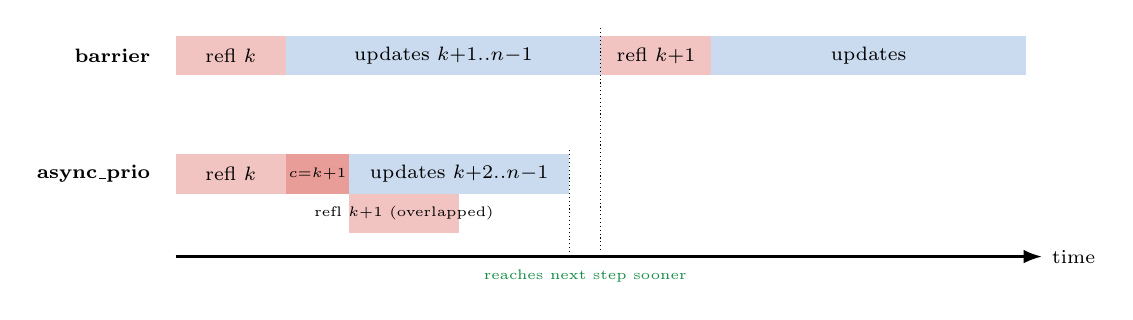
\begin{tikzpicture}[font=\scriptsize,>=Latex]
  % barrier
  \node[anchor=east] at (-0.2,0){\textbf{barrier}};
  \onslide<1->{\fill[critcol!30](0,-0.25)rectangle(1.4,0.25);\node at(0.7,0){refl $k$};}
  \onslide<1->{\fill[workcol!25](1.4,-0.25)rectangle(5.4,0.25);\node at(3.4,0){updates $k{+}1..n{-}1$};}
  \onslide<1->{\fill[critcol!30](5.4,-0.25)rectangle(6.8,0.25);\node at(6.1,0){refl $k{+}1$};}
  \onslide<1->{\fill[workcol!25](6.8,-0.25)rectangle(10.8,0.25);\node at(8.8,0){updates};}
  % async_prio
  \node[anchor=east] at (-0.2,-1.5){\textbf{async\_prio}};
  \onslide<2->{\fill[critcol!30](0,-1.75)rectangle(1.4,-1.25);\node at(0.7,-1.5){refl $k$};}
  \onslide<3->{\fill[critcol!50](1.4,-1.75)rectangle(2.2,-1.25);\node at(1.8,-1.5){\tiny $c{=}k{+}1$};}
  \onslide<4->{\fill[workcol!25](2.2,-1.75)rectangle(5.0,-1.25);\node at(3.6,-1.5){updates $k{+}2..n{-}1$};}
  \onslide<4->{\fill[critcol!30](2.2,-2.25)rectangle(3.6,-1.75);\node at(2.9,-2.0){\tiny refl $k{+}1$ (overlapped)};}
  \onslide<5->{\draw[densely dotted](5.4,0.35)--(5.4,-2.5);
               \draw[densely dotted](5.0,-1.2)--(5.0,-2.5);
               \node[okgreen] at (5.2,-2.8){\tiny reaches next step sooner};}
  \draw[->,thick](0,-2.55)--(11,-2.55) node[right]{time};
\end{tikzpicture}
\vfill
\small
\begin{itemize}
  \item<3-> driver does the \crit{critical column $k{+}1$} itself, on a briefly-held HVX context;
  \item<4-> then builds reflector $k{+}1$ \emph{underneath} the workers' updates of $k{+}2..n{-}1$;
  \item<5-> the per-step critical path shrinks $\Rightarrow$ wins most when there are many reflectors.
\end{itemize}
\end{frame}

% ===============================================================
%  HVX CONTEXT ALLOCATION
% ===============================================================
\begin{frame}{The scarce resource: 4 HVX contexts}
\centering
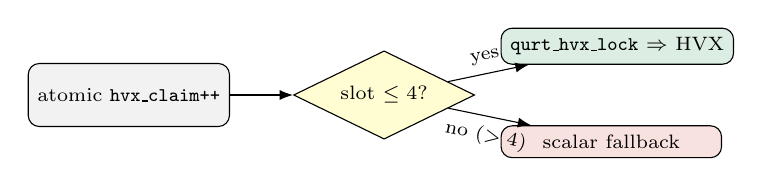
\begin{tikzpicture}[font=\scriptsize,>=Latex,node distance=5mm]
  \node[draw,rounded corners,fill=gray!10,minimum height=8mm] (c){atomic \texttt{hvx\_claim++}};
  \node[draw,diamond,aspect=2,fill=yellow!18,right=8mm of c,minimum width=2.3cm](t){slot $\le 4$?};
  \node[draw,rounded corners,fill=okgreen!15,above right=1mm and 9mm of t,minimum width=2.8cm](h){\texttt{qurt\_hvx\_lock} $\Rightarrow$ HVX};
  \node[draw,rounded corners,fill=critcol!15,below right=1mm and 9mm of t,minimum width=2.8cm](s){scalar fallback};
  \draw[->](c)--(t);
  \onslide<2->{\draw[->](t)-- node[above,sloped]{yes}(h);}
  \onslide<3->{\draw[->](t)-- node[below,sloped]{no ($>4$)}(s);}
\end{tikzpicture}
\vfill
\small
\begin{itemize}
  \item<1-> each worker claims a slot with \emph{one} atomic increment (race-free);
  \item<2-> the first $\le 4$ claimants get a real vector context;
  \item<3-> surplus workers (when $n_t>4$) do the \emph{same} math in scalar --- graceful, no blocking.
\end{itemize}
\onslide<4->{\footnotesize\centering (Aside: \texttt{qurt\_hvx\_try\_lock} is a trap on
v65+ --- it grants nothing, silently dropping all workers to scalar.)}
\end{frame}

% ===============================================================
%  RESULTS
% ===============================================================
\begin{frame}{Measured results (Hexagon ISS, \texttt{c15:14}, $n_t{=}4$)}
\onslide<1->{
\textbf{Square matrices --- the reduction dominates; scheduling policy is a wash:}
\begin{center}\small
\begin{tabular}{lrr}
\toprule
variant / mode & $128^2$ & $256^2$\\\midrule
\texttt{v0\_pool} (scalar reduce) & 341{,}377 & 938{,}095\\
\texttt{v1} (+HVX reduction)      & 301{,}989 & 792{,}991\\
\texttt{v7} barrier               & 287{,}766 & 735{,}121\\
\texttt{v7} async\_prio           & 289{,}327 & 724{,}195\\\midrule
\textit{policy (barrier vs prio)} & $+0.5\%$ & $-1.5\%$\\
\bottomrule
\end{tabular}
\end{center}}
\onslide<2->{
\textbf{Tall-skinny --- here scheduling \emph{policy} pays off (up to $1.29\times$):}
\begin{center}\small
\begin{tabular}{lrrr}
\toprule
$m\times n$ & async\_prio & barrier & speedup\\\midrule
$1024\times16$ & 268{,}663 & 303{,}529 & $1.13\times$\\
$1024\times32$ & 430{,}811 & 514{,}201 & $1.19\times$\\
$1024\times64$ & 658{,}439 & 846{,}695 & $\mathbf{1.29\times}$\\
$2048\times32$ & 772{,}987 & 953{,}679 & $1.23\times$\\
\bottomrule
\end{tabular}
\end{center}}
\end{frame}

% ===============================================================
\begin{frame}{Takeaways}
\begin{enumerate}\itemsep6pt
  \item The \crit{register-only reduction} is the biggest single lever ($\sim$70\% of the square-matrix gain).
  \item \crit{Critical-path pivot overlap} is shape-conditioned: neutral on square,
        up to $1.29\times$ on tall-skinny (least-squares) QR --- and it grows with $n$
        (more reflectors to hide).
  \item The \crit{HVX context}, not the thread, is the binding resource: budget it,
        degrade to scalar past 4 threads.
\end{enumerate}
\vfill
\centering\small Source: \texttt{v7\_dag\_hvx\_sched.c}\quad$\cdot$\quad
companion report: \texttt{docs/v7\_dag\_hvx\_sched.pdf}
\end{frame}

\end{document}
